%%%%%%%%%%%%%%%%%%%%%%% file template.tex %%%%%%%%%%%%%%%%%%%%%%%%%
%
% This is a general template file for the LaTeX package SVJour3
% for Springer journals.          Springer Heidelberg 2010/09/16
%
% Copy it to a new file with a new name and use it as the basis
% for your article. Delete % signs as needed.
%
% This template includes a few options for different layouts and
% content for various journals. Please consult a previous issue of
% your journal as needed.
%
%%%%%%%%%%%%%%%%%%%%%%%%%%%%%%%%%%%%%%%%%%%%%%%%%%%%%%%%%%%%%%%%%%%
%
% First comes an example EPS file -- just ignore it and
% proceed on the \documentclass line
% your LaTeX will extract the file if required
% \begin{filecontents*}{example.eps}
% %!PS-Adobe-3.0 EPSF-3.0
% %%BoundingBox: 19 19 221 221
% %%CreationDate: Mon Sep 29 1997
% %%Creator: programmed by hand (JK)
% %%EndComments
% gsave
% newpath
%   20 20 moveto
%   20 220 lineto
%   220 220 lineto
%   220 20 lineto
% closepath
% 2 setlinewidth
% gsave
%   .4 setgray fill
% grestore
% stroke
% grestore
% \end{filecontents*}
%
\RequirePackage{fix-cm}
%
\documentclass{svjour3}                     % onecolumn (standard format)
% \documentclass[smallcondensed]{svjour3}     % onecolumn (ditto)
% \documentclass[smallextended]{svjour3}       % onecolumn (second format)
% \documentclass[twocolumn]{svjour3}          % twocolumn
%
\smartqed  % flush right qed marks, e.g. at end of proof
%
\usepackage{graphicx}
%
% \usepackage{mathptmx}      % use Times fonts if available on your TeX system
%
% insert here the call for the packages your document requires
%\usepackage{latexsym}
\usepackage{physics}
\usepackage{hyperref}
% \usepackage{clevref}
\usepackage{lineno}
\usepackage{siunitx}        % to use accurate number and unit
\usepackage{xparse}         % to use accurate number and unit

% \usepackage{cleveref}
% \usepackage{scalerel}
% \usepackage{tikz}
% \usepackage{orcidlink}
% etc.
%
% please place your own definitions here and don't use \def but
% \newcommand{}{}
\newcommand*{\bkt}[1]{\left(#1\right)}
\newcommand*{\Bkt}[1]{\left[#1\right]}
\newcommand*{\BKT}[1]{\left\{#1\right\}}

% \newcommand{\orcid}[1]{\href{https://orcid.org/#1}{\textcolor[HTML]{A6CE39}{\aiOrcid}}}
%
% Insert the name of "your journal" with
% \journalname{myjournal}
%
\begin{document}

\title{Analysis of two-dimensional non-linearly propagating waves in a very large floating solar panel%\thanks{Grants or other notes
%about the article that should go on the front page should be
%placed here. General acknowledgments should be placed at the end of the article.}
}
% \subtitle{Do you have a subtitle?\\ If so, write it here}

%\titlerunning{Short form of title}        % if too long for running head

\author{Pengpeng Xu       
        \and
        Peter R. Wellens %etc.
}

%\authorrunning{Short form of author list} % if too long for running head

\institute{Pengpeng Xu \and Peter R. Wellens*
            \at
            Maritime and Transport Technology Department, Delft University of Technology, Mekelweg 2, 2628 CD, The Netherland\\
            %   *Tel.: +31-6-51672361\\
            *\email{\href{mailto:p.r.wellens@tudelft.nl}{p.r.wellens@tudelft.nl}}          %  \\
%             \emph{Present address:} of F. Author  %  if needed
        %   \and
        %   Peter R. Wellens \at
        %       second address
}

\date{Received: date / Accepted: date}
% The correct dates will be entered by the editor


\maketitle

\linenumbers

\begin{abstract}
This article analyzes the non-linear wave propagation in the fluid-structure interaction (FSI) model of a very large floating structure. The multi-time-scale perturbation method with the introduction of the wave steepness as the perturbation leads to hierarchic equations. Up to the moderate-high range, the solution shows that the plane progressive wave remains its linear property and is corrected by the non-linearity, showing amplitudes dispersion in term of the second-order.
\keywords{Nonlinear wave \and FSI \and Bernoulli-Euler-von K\'{a}rm\'{a}n beam \and VLFS.}
% \PACS{PACS code1 \and PACS code2 \and more}
% \subclass{MSC code1 \and MSC code2 \and more}
\end{abstract}

\section{Introduction}
\label{sec:1}
\cite{Ma2020} gives two-dimensional (2D) analytical solution to the fluid-structure interaction (FSI) model of very large floating structures (VLFS), in which the non-linear water wave is coupled with the linear Euler-Bernoulli beam. 

\cite{Jang2013} introduces a new integral approach to solve the non-linear Euler-Bernoulli-von K\'{a}rm\'{a}n beam.

\cite{Vanden-Broeck2011} derives the non-linear waves travelling in infinitely long floating ice floes with an adopted Stokes expansion. The non-linearity is due to the ice non-linear stiffness that involves non-linear calculation of curvature and also the non-linear water potential. The structural dynamic is neglected. 

\cite{D.Wang2002} gives the solution of linear FSI waves in floating plates in both infinite and finite domains. The finite domain problem is numerically solved by the boundary element method.

Our hypothesises are i). the geometrical non-linearity is a small term in terms of wave amplitude and ii). it corrects the dispersion relation. With the first hypothesis, the wave propagation shall maintain the major linear properties. With the second hypothesis, the non-linearity shall correct the wave propagation with the scale of wave amplitude. 

\section{Theoretical model}
\label{sec:2}
Fig.~\ref{fig:sketch} shows the sketch of the model, in which a large offshore solar panel floats on the sea surface in an infinite open area. Compared with the wave length, the structural length is so large that it can be seen as a infinite domain. The assumptions are that a). the structure is impenetrable for both the beneath water and the above air and b). vacuum does not occur. Therefore the solar panel can be modeled as a two-dimensional (2D) von K\'{a}rm\'{a}n plate that contains only the geometrical non-linearity. In the 2D case, the 1D Euler-Bernoulli-von K\'{a}rm\'{a}n beam models the geometrically non-linear structure. The linear potential theory describes the water motion and the hydrodynamics. A train of waves travelling in an arbitrary direction, e.g., rightwards, address the investigation of the fluid-structure interaction (FSI).

\begin{figure}
    % \centering
    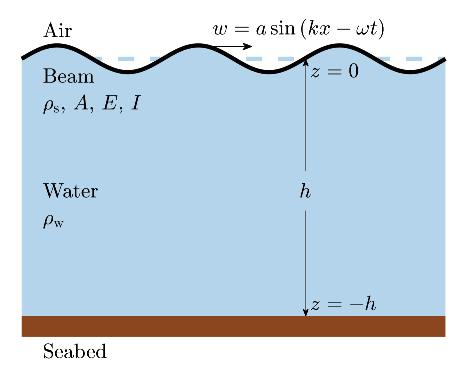
\includegraphics[width=0.5\columnwidth]{sketch.eps}
    \caption{A vary large ocean solar panel float on the sea surface. }
    \label{fig:sketch}
\end{figure}

\subsection{Governing equations}
\subsubsection{Nonlinear Euler-Bernoulli-von K\'{a}rm\'{a}n theory for beam}
The equation of motion (EOM) of the nonlinear Euler-Bernoulli-von K\'{a}rm\'{a}n beam reads
\begin{equation}
    \rho_\mathrm{s} A \pdv[2]{w}{t} 
    + E I \pdv[4]{w}{x} 
    - \frac{3}{2} A E \bkt{\pdv{w}{t}}^2\pdv[2]{w}{t}
    = q_\mathrm{w}.
    \label{eq: beam}
\end{equation}

The beam is of material density \ensuremath{\rho_\mathrm{s}}, cross-section area \ensuremath{A=bd}, Young's module \ensuremath{E} and inertial moment \ensuremath{I=\frac{bd^3}{12}}. Here \ensuremath{d} stands for the beam thickness (in \ensuremath{z}-direction), while \ensuremath{b} for the beam width (in \ensuremath{y}-direction that is neglected in 2D model). The water has density of \ensuremath{\rho_\mathrm{w}} and the uniform depth of \ensuremath{h}. \ensuremath{w} is the transverse displacement of beam. The external distributed load \ensuremath{q} is only the hydro-dynamic load because the floating equilibrium state sets off beam's gravity and buoyancy. \ensuremath{q} has the unit of \ensuremath{\Bkt{\si[per-mode=symbol]{\newton\per\meter}}} because the load is distributed over length in the 1D beam model.

\subsubsection{Liner potential theory for water}
The linear potential theory gives governing equations of inviscid, irrotational and incompressible fluid
\begin{equation}
    \pdv[2]{\phi}{x} + \pdv[2]{\phi}{z} = 0,
    \label{eq: laplace}
\end{equation}
where \ensuremath{\phi} represents the fluid velocity potential. 

At the bottom \ensuremath{z=-h}, the seabed is impenetrable: 
\begin{equation}
    \pdv{\phi}{z} = 0 \qq{at} z=-h,
    \label{eq: bottom}
\end{equation}
where \ensuremath{h} is the uniform water depth. 

At the free surface \ensuremath{z=0}, the kinematic boundary condition reads
\begin{equation}
    \pdv{\eta}{t} = \pdv{\phi}{z} \qq{at} z=0,
    \label{eq: surface kinematic bc}
\end{equation}
where \ensuremath{\eta} stands for the free surface elevation. And the Bernoulli equation gives the dynamic boundary condition:
\begin{equation}
    p + \rho_\mathrm{w} \pdv{\phi}{t} + \rho_\mathrm{w} \mathrm{g} \eta = 0 \qq{at} z = 0,
    \label{eq: surface dynamic bc}
\end{equation}
where \ensuremath{p} is the water pressure with unit \ensuremath{\Bkt{\si[per-mode=symbol]{\newton\per\meter\squared}}}, and \ensuremath{\mathrm{g}=\SI[per-mode=symbol]{9.81}{\Bkt{\meter\per\second\squared}}} is acceleration of gravity.

\subsubsection{FSI equations}
The beam and water models are coupled through the interface boundary conditions:
\begin{equation}
    w = \eta \qq{and} q_\mathrm{w} = p b \qq{at} z = 0.
    \label{eq: interface bc}
\end{equation}
Note that the force condition calculates the hydro-load by multiplying hydro-pressure \ensuremath{p} with beam width \ensuremath{b} for the consistence of unit \ensuremath{\Bkt{\si[per-mode=symbol]{\newton\per\meter}}}.

Now the fluid and structure governing equations are coupled at the free surface \ensuremath{z=0}:
\begin{equation}
    \pdv{w}{t} = \pdv{\phi}{z} 
    \label{eq: FSI kinematic}
\end{equation}
and
\begin{equation}
    \pdv[2]{w}{t} 
    + \beta \pdv[4]{w}{x} 
    - \frac{18\beta}{d^2} \bkt{\pdv{w}{t}}^2\pdv[2]{w}{t}
    + \alpha \pdv{\phi}{t} 
    + \alpha \mathrm{g} w 
    = 0,
    \label{eq: FSI EOM}
\end{equation}
where \ensuremath{\alpha} and \ensuremath{\beta} are two parameter ratios given by 
\begin{equation}
    \alpha = \frac{\rho_\mathrm{w}}{ \rho_\mathrm{b} d }
\end{equation}
and
\begin{equation}
    \beta = \frac{ d^2 E_\mathrm{b} }{ 12 \rho_\mathrm{b} }.
\end{equation}
Here, \ensuremath{A} \ensuremath{I} and \ensuremath{b} have been replaced or eliminated by \ensuremath{A=bd}, \ensuremath{I=\frac{bd^3}{12}} and Eq.~\eqref{eq: interface bc}.


\subsection{Non-dimensionalization}
Introduce new variables
\begin{equation}
    \left\{
    \begin{aligned}
        & X = k x \\
        & Z = k z \\
        & T = \sqrt{ k \tanh\bkt{kh} } \,  t \\
        & W\bkt{X,T} = \frac{w\bkt{X,T}}{a} \\
        & \Phi\bkt{X,Z,T} = \frac{ \sqrt{ k \tanh\bkt{kh} } }{ a \mathrm{g} } \phi\bkt{X,Z,T} \\
        & H = k h \\
        & \varepsilon = k a
    \end{aligned}
    \right.
    \label{eq: nondimensional variables}
\end{equation}
where \ensuremath{a} and \ensuremath{k} are the wave amplitude and wave number, respectively. The scaled time \ensuremath{T} is introduced partly for non-dimension (it is not completely dimensionless) and partly for easy multiplication. Note that the perturbation \ensuremath{\varepsilon} actually represents the wave steepness. 

Substitution of Eq.~\eqref{eq: nondimensional variables} into Eqs.~\eqref{eq: FSI kinematic} and \eqref{eq: FSI EOM} yields the non-dimensional EOM for the non-linear FSI governing equations at free surface \ensuremath{Z=0}:
\begin{equation}
    \pdv{W}{T} = \pdv{\Phi}{z}
    \label{eq: FSI kinematic nondimension}
\end{equation}
and
\begin{equation}
    k \tanh\bkt{H} \pdv[2]{W}{T}
    + \beta k^4 \pdv[4]{W}{X}
    - \varepsilon^2 18 \frac{ \beta k^2 }{ d^2 } \bkt{ \pdv{W}{X} }^2 \pdv[2]{W}{X} 
    + \alpha \mathrm{g} \pdv{\Phi}{T} 
    + \alpha \mathrm{g} W
    = 0
    \label{eq: FSI EOM nondimension}
\end{equation}

Eq.~\eqref{eq: FSI EOM nondimension} demonstrates that the non-linear term is of high order \ensuremath{\order{\varepsilon^2}}. In other words, the wave amplitude squared \ensuremath{a^2} scales the non-linearity. The non-linear effect become significant for the moderate-large waves, which suffices the requirement of the von K\'{a}rm\'{a}n theory. 



\section{Analytical solution}
\label{sec:3}
\subsection{Multi-time-scale}
Introduce the multi-time-scale with two-term expansion:
\begin{equation}
    T \sim T_0 + \varepsilon^2 T_1.
    \label{eq: expand time}
\end{equation}

Eq.~\eqref{eq: expand time} also expands partial differential operators about time \ensuremath{T}
\begin{equation}
    \pdv{}{T} \sim \pdv{}{T_0} + \varepsilon^2 \pdv{}{T_1}
    \label{eq: expand time dt}
\end{equation}
and
\begin{equation}
    \pdv{}{T} \sim \pdv[2]{}{T_0} + 2 \varepsilon^2 \pdv{}{T_0}{T_1} + \order{\varepsilon^4}
    \label{eq: expand time ddt}
\end{equation}

The undetermined solution of plane wave \ensuremath{W\bkt{X,T}} is expanded accordingly
\begin{equation}
    W\bkt{X,T} = W\bkt{X,T_0,T_1} \sim W_0\bkt{X,T_0,T_1} + \varepsilon^2 W_1\bkt{X,T_0,T_1} 
    \label{eq: expand solution}
\end{equation}

Note that the water potential is linear and thus needing no expansion
\begin{equation}
    \Phi\bkt{X,Z,T} = \Phi\bkt{X,Z,T_0,T_1}.
\end{equation}


\subsection{Hierarchical equations}
Substituting Eqs.~(\ref{eq: expand time}-\ref{eq: expand solution}) into Eqs.~\eqref{eq: FSI kinematic nondimension} and \eqref{eq: FSI EOM nondimension} and collecting \ensuremath{\varepsilon}, the classic perturbation procedure generates a series of hierarchical linear partial differential equations (PDE) with non-linear in-homogeneous terms on the right hind side from the second-order on. Retain up to the second-order:

\begin{itemize}
    \item \ensuremath{\order{\varepsilon^0}}:
    
    \begin{equation}
        \pdv{W_0}{T_0}
        =
        \frac{\mathrm{g}}{\tanh\bkt{H}} \pdv{\Phi}{Z} \eval_{Z=0}
        \label{eq: 1st order kinematic}
    \end{equation}
    
    \begin{equation}
    \begin{aligned}
        \beta\,{k}^{4} {\frac { \partial ^{4} W_0 }{\partial {X}^{4}}} 
        + k\tanh \left( H \right) {\frac {\partial ^{2}  W_0 }{\partial {T_0}^2}}
        + \alpha\mathrm{g}{\frac {\partial \Phi }{\partial T_0}} \eval_{Z=0}
        + \alpha\mathrm{g} W_0
        =0
    \end{aligned}
    \label{eq: 1st order combined}
    \end{equation}
    
    \begin{equation}
        \pdv[2]{\Phi}{X} + \pdv[2]{\Phi}{Z} = 0
        \label{eq: Laplace demensionless}
    \end{equation}
    
    \begin{equation}
        \pdv{\Phi}{Z} \eval_{Z=-H} = 0
        \label{eq: seabed demensionless}
    \end{equation}
    
    \item \ensuremath{\order{\varepsilon^2}}:
    
    \begin{equation}
    \begin{aligned}
        k & \tanh\bkt{H} \pdv[2]{W_1}{T_0}
        + \beta k^4 \pdv[4]{W_1}{X}
        + \alpha \mathrm{g} W_1  
        \\
        & =
        18 \frac{\beta k^4}{d^2} \Bkt{\pdv{W_0}{X}}^2 \pdv[2]{W_0}{X}
        - 2 k \tanh \bkt{H} \pdv{W_0}{T_0}{T_1}
        - \alpha \mathrm{g} \pdv{\Phi}{T_1} \eval_{Z=-H}
    \end{aligned}
    \label{eq: 2nd order combined}
    \end{equation}
\end{itemize}


\subsection{The first-order}

\subsubsection{The non-dimensional first-order solution}
First separate the potential into three parts, namely the time-dependent part \ensuremath{\varphi\bkt{T_0,t_1}}, the horizontal space-dependent part \ensuremath{\xi\bkt{X}} and the vertical space-dependent part as \ensuremath{\zeta\bkt{Z}}
\begin{equation}
    \Phi\bkt{X,Z,T_0,T_1} = \varphi\bkt{T_0,T_1} \xi\bkt{X} \zeta\bkt{Z}.
    \label{eq: phi separation}
\end{equation}

Substitution of Eq.~\eqref{eq: phi separation} into Eqs.~\eqref{eq: Laplace demensionless} and \eqref{eq: seabed demensionless} and elimination of \ensuremath{\varphi\bkt{T_0,T_1}} yeild
\begin{equation}
    \Phi\bkt{X,Z,T_0,T_1} = \varphi\bkt{T_0,T_1}  \cos \bkt{ X } \cosh\bkt{Z+H}.
    \label{eq: sol xi and zeta}
\end{equation}
Note that the integral constants of \ensuremath{\xi\bkt{X}} and \ensuremath{\zeta\bkt{Z}} merge into the undetermined time-dependent function \ensuremath{\varphi\bkt{T_0,T_1}}. We also get rid of the the arbitrary phase shift of \ensuremath{\xi\bkt{X}} because only the plane propagating wave is of interest. 

Taking the partial differentiation about \ensuremath{T_0} of Eq.~\eqref{eq: 1st order combined} and using Eqs.~\eqref{eq: 1st order kinematic} and \eqref{eq: sol xi and zeta}, we obtain
\begin{equation}
    k \tanh\bkt{H} \pdv[2]{\varphi}{T_0} + \beta k^4 \varphi + \alpha \pdv[2]{\varphi}{T_0} + \alpha \mathrm{g} \varphi = 0.
    \label{eq: ode for varphi}
\end{equation}

The solution of Eq.~\eqref{eq: ode for varphi} is
\begin{equation}
    \varphi \bkt{T_0,T_1}
    = 
    C\bkt{T_1}
    \cos \bkt{ 
    \sqrt{\frac{ \beta k^4 + \alpha \mathrm{g} }{ k \tanh\bkt{H} + \alpha }} T_0 
    + \theta\bkt{T_1}
    }.
    \label{eq: sol varphi}
\end{equation}

The coefficient in front of the regular time scale \ensuremath{T_0} in Eq.~\eqref{eq: sol varphi} is the primary angular frequency \ensuremath{\Omega_0}
\begin{equation}
    \Omega_0 = \sqrt{ \frac{ \beta k^4 + \alpha \mathrm{g} }{ k \tanh\bkt{H} + \alpha } }
    \label{eq: linear DR}
\end{equation}

Eq.~\eqref{eq: linear DR} is the non-dimensional linear dispersion relation.

Combine Eqs.~\eqref{eq: sol xi and zeta} and \eqref{eq: sol varphi} into a right-ward propagating wave as shown in Fig.~\ref{fig:sketch} 
\begin{equation}
    W_0 \left( X,T_{0},T_{1} \right) 
    = 
    A \bkt{T_1}
    \sin\bkt{ X
    - \Omega_0 T_0 
    + \theta\bkt{T_1} }
    \label{eq: sol W0}
\end{equation}
and
\begin{equation}
    \Phi\bkt{X,Z,T_0,T_1} 
    = 
    - \Omega_0
    \frac{ \cosh\bkt{Z+H} }{ \sinh\bkt{H} } 
    A\bkt{T_1} 
    \cos \bkt{ 
    X
    - \Omega_0 T_0 
    + \theta\bkt{T_1}
    }
    \label{eq: sol Phi}
\end{equation}
where \ensuremath{A\bkt{T_1}=- \frac{\sinh\bkt{H}}{\Omega_0}  C\bkt{T_1}}.

\subsubsection{The dimensional first-order solution}
Inverse utilization of Eq.~\eqref{eq: nondimensional variables} gives the dimensional first-order solution.
\begin{itemize}
    \item The dimensional first-order dispersion relation
    \begin{equation}
        \omega_0 =  \sqrt{ \frac{ k \tanh\bkt{kh} \bkt{\beta k^4 + \alpha \mathrm{g} } }{ k \tanh\bkt{kh} + \alpha } }
        \label{eq: linear dr}
    \end{equation}
    
    \item The dimensional first-order phase velocity
\begin{equation}
    c = \sqrt{ \frac{ \tanh\bkt{kh} \bkt{\beta k^4 + \alpha \mathrm{g} } }{ k \bkt{ k \tanh\bkt{kh} + \alpha } } }
\end{equation}
\end{itemize}


\subsection{The second-order}
\subsubsection{The non-dimensional second-order solution}
Substitute the first-order solution Eqs.~\eqref{eq: sol Phi} and \eqref{eq: sol W0} into the right-hand-side of Eq.~\eqref{eq: 2nd order combined}, then collect the trigonometric. There exist primary trigonometric terms, i.e., \ensuremath{\sin\bkt{ X - \Omega_0 T_0 + \theta\bkt{T_1}}} and \ensuremath{\cos\bkt{ X - \Omega_0 T_0 + \theta\bkt{T_1}}}. Their coefficients are
\begin{equation}
    \begin{aligned}
        C_{\sin}
        = & 
        {\frac {2\,k\tanh \left( H \right) \sqrt {\beta\,{k}^{4}+\alpha\mathrm{g}} }{\sqrt {k\tanh \left( H \right) +\alpha}}}  A \left( T_{1} \right)  {\frac {{\rm d} \theta \left( T_{1} \right)}{{\rm d}T_{1}}}
        + {\frac {9\,\beta\,{k}^{2} }{2\,{d}^{2}}}  A^{3}  \left( T_{1} \right)  \\
        & + \frac {\cosh \left( H \right) \alpha\mathrm{g} }{\sinh \left( H \right) }   {\frac {\sqrt {\beta\,{k}^{4}+\alpha\mathrm{g}}}{\sqrt {k\tanh \left( H \right) +\alpha}}}  A \left( T_{1} \right) {\frac {{\rm d} \theta \left( T_{1} \right)}{{\rm d}T_{1}}}
    \end{aligned}
    \label{eq: coef sin}
\end{equation}

\begin{equation}
    \begin{aligned}
        C_{\cos}
        = & 
        2\,{\frac {k\tanh \left( H \right)   \sqrt {\beta\,{k}^{4}+\alpha\mathrm{g}}}{\sqrt {k\tanh \left( H \right) +\alpha}}}   {\frac {{\rm d} A \left( T_{1} \right)}{{\rm d}T_{1}}}   \\
        & + \frac {\cosh \left( H \right) \alpha\mathrm{g} }{\sinh \left( H \right) } 
        {\frac {\sqrt {\beta\,{k}^{4}+\alpha\mathrm{g}}}{\sqrt {k\tanh \left( H \right) +\alpha}}}  \frac {{\rm d} A \left( T_{1} \right)}{{{\rm d} }T_{1}}
    \end{aligned}
    \label{eq: coef cos}
\end{equation}

Avoiding secular terms requires that the \ensuremath{C_{\sin}} and \ensuremath{C_{\cos}} equal to zero. Eq.~\eqref{eq: coef cos} can solve \ensuremath{A\bkt{T_1}}:
\begin{equation}
    A\bkt{T_1} = A.
    \label{eq: sol C4}
\end{equation}
Hence A is a arbitrary non-dimensional constant independent of the slow time-scale \ensuremath{T_1}.

Substitution of Eq.~\eqref{eq: sol C4} into Eq.~\eqref{eq: coef sin} leads to
\begin{equation}
    \theta \left( T_{1} \right) 
    = 
    -\frac {9\,\beta\,{k}^{2}  \sinh \left( 2\,H \right) }{2\,{d}^{2} \left( \alpha\mathrm{g}\cosh \left( 2\,H \right) +2\,k\cosh \left( 2\,H \right) +\alpha\mathrm{g}-2\,k \right) \Omega_0 }
    {A}^{2} T_{1}.
    \label{eq: theta2}
\end{equation}

Substitute Eqs.~\eqref{eq: sol C4} and \eqref{eq: theta2} back into the first-order solution Eq.~\eqref{eq: sol W0}, and let \ensuremath{A=1}. Now, the plane propagating wave reads

\begin{equation}
    \begin{aligned}
    W_{0}
    =
    \sin\bkt{ X
    - \Omega_0 T
    -\frac {9\varepsilon^2 \beta{k}^{2}  \sinh \left( 2H \right) T }{2{d}^{2} \left( \alpha \mathrm{g} \cosh \left( 2H \right) +2k\cosh \left( 2H \right) +\alpha \mathrm{g}-2k \right) \Omega_0 }
     } .
    \end{aligned}
    \label{eq: sol W0 2nd}
\end{equation}

The nonlinear angular frequency up to the second-order is
\begin{equation}
    \begin{aligned}
        \Omega 
        =
        \Omega_0 + \frac {9\varepsilon^2 \beta{k}^{2}  \sinh \left( 2H \right) }{2{d}^{2} \left( \alpha \mathrm{g} \cosh \left( 2H \right) +2k\cosh \left( 2H \right) +\alpha \mathrm{g}-2k \right) \Omega_0 }.
    \end{aligned}
    \label{eq: sol Omega 2nd}
\end{equation}


\subsubsection{The dimensional second-order solution}
Inverse utilization Eq.~\eqref{eq: nondimensional variables} gives the dimensional second-order solution, too.
\begin{itemize}
    \item The dimensional second-order dispersion relation
    \begin{equation}
    \begin{aligned}
        \omega 
        = & 
        \sqrt {\frac {{\beta\,{k}^{4}+\alpha\mathrm{g}}}{ {k\tanh \left( kh \right) +\alpha}}} 
        + 
        \frac{ 9 \varepsilon^2 \beta k^2 \tanh\bkt{kh} }{ 2 d^2 \bkt{ 2 k \tanh^2\bkt{kh} + \alpha \mathrm{g} } }
        \sqrt{\frac
        {k\tanh \left( kh \right) +\alpha}
        {\beta{k}^{4}+\alpha\mathrm{g}} }
    \end{aligned}
    \label{eq: 2.34}
\end{equation}
    
    \item The dimensional second-order phase velocity
    \begin{equation}
    \begin{aligned}
        c 
        = & 
        \frac{1}{k} \sqrt {\frac {{\beta\,{k}^{4}+\alpha\mathrm{g}}}{ {k\tanh \left( kh \right) +\alpha}}} 
        + 
        \frac{ 9 \varepsilon^2 \beta k \tanh\bkt{kh} }{ 2 d^2 \bkt{ 2 k \tanh^2\bkt{kh} + \alpha \mathrm{g} } }
        \sqrt{\frac
        {k\tanh \left( kh \right) +\alpha}
        {\beta{k}^{4}+\alpha\mathrm{g}} }
    \end{aligned}
\end{equation}
\end{itemize}

\section{Discussion}
\label{sec:4}
\input{Sections/section4}

\section{Conclusion}
\label{sec:5}
\input{Sections/section5}

\section*{Acknowledgement}
\label{sec:6}
This research is financially supported by the China Scholarship Council with the project NO. 201707720039.



%\begin{acknowledgements}
%If you'd like to thank anyone, place your comments here
%and remove the percent signs.
%\end{acknowledgements}


% Authors must disclose all relationships or interests that 
% could have direct or potential influence or impart bias on 
% the work: 
%
% \section*{Conflict of interest}
%
% The authors declare that they have no conflict of interest.


% BibTeX users please use one of
% \bibliographystyle{spbasic}      % basic style, author-year citations
\bibliographystyle{spmpsci}      % mathematics and physical sciences
% \bibliographystyle{spphys}       % APS-like style for physics
\bibliography{references.bib}   % name your BibTeX data base

% % Non-BibTeX users please use
% \begin{thebibliography}{}
% %
% % and use \bibitem to create references. Consult the Instructions
% % for authors for reference list style.
% %
% \bibitem{RefJ}
% % Format for Journal Reference
% Author, Article title, Journal, Volume, page numbers (year)
% % Format for books
% \bibitem{RefB}
% Author, Book title, page numbers. Publisher, place (year)
% % etc
% \end{thebibliography}

\end{document}
% end of file template.tex

